\documentclass{overture}
%**********************************************************
%
% Bibliography support
%
%**********************************************************
%\def\@reportno{YY--NN}		% default report no.
%\def\reportno#1{\gdef\@reportno{#1}}

\newcommand{\bthisbibliography}[1]{\section*{References}%
   \begin {list} {}%
     {\settowidth {\labelwidth} {[#1]XX}%
      \setlength {\leftmargin} {\labelwidth}%
      \addtolength{\leftmargin} {\labelsep}%
      \setlength {\parsep} {1ex}%
      \setlength {\itemsep} {2ex}%
     }
  }
\newcommand{\ethisbibliography}{\end{list}}
\newcommand{\refitem}[2]
  {\bibitem[#1]{#2}}

\newcommand{\back}{$\setminus$}
\newcommand{\RuleTarget}[1]{\hypertarget{rule:#1}{}}
\newcommand{\Ruledef}[2]
{
  \RuleTarget{#1}\Rule{#1}{#2}%
  }
\newcommand{\Ruleref}[1]{
  \hyperlink{rule:#1}{#1}}
\newcommand{\Lit}[1]{`{\tt #1}\Quote}
\newcommand{\Rule}[2]{
  \begin{quote}\begin{tabbing}
    #1\index{#1}\ \ \= = \ \ \= #2  ; %    Adds production rule to index
    
  \end{tabbing}\end{quote}
  }
\newcommand{\SeqPt}[1]{\{\ #1\ \}}
\newcommand{\lfeed}{\\ \> \>}
\newcommand{\dsepl}{\ $|$\ }
\newcommand{\dsep}{\\ \> $|$ \>}
\newcommand{\Lop}[1]{`{\sf #1}\Quote}
\newcommand{\blankline}{\vspace{\baselineskip}}
\newcommand{\Brack}[1]{(\ #1\ )}
\newcommand{\nmk}{\footnotemark}
\newcommand{\ntext}[1]{\footnotetext{{\bf Note: } #1}}
\newlength{\kwlen}
\newcommand{\Keyw}[1]{\settowidth{\kwlen}{\tt #1}\makebox[\kwlen][l]{\sf
    #1}}
\newcommand{\keyw}[1]{{\sf #1}}
\newcommand{\id}[1]{{\tt #1}}
\newcommand{\metaiv}[1]{\begin{alltt}\input{#1}\end{alltt}}

\newcommand{\OptPt}[1]{[\ #1\ ]}
\newcommand{\MAP}[2]{\kw{map }#1\kw{ to }#2}
\newcommand{\INMAP}[2]{\kw{inmap }#1\kw{ to }#2}
\newcommand{\SEQ}[1]{\kw{seq of }#1}
\newcommand{\NSEQ}[1]{\kw{seq1 of }#1}
\newcommand{\SET}[1]{\kw{set of }#1}
\newcommand{\PROD}[2]{#1 * #2}
\newcommand{\TO}[2]{$#1 \To #2$}
\newcommand{\FUN}[2]{#1 \To #2}
\newcommand{\PUBLIC}{\ifthenelse{\boolean{VDMpp}}{public\mbox{}}{\mbox{}}}
\newcommand{\PRIVATE}{\ifthenelse{\boolean{VDMpp}}{private}{\mbox{}}}
\newcommand{\PROTECTED}{\ifthenelse{\boolean{VDMpp}}{protected}{\mbox{}}}

\usepackage{graphicx, color}

% definition of VDM++, JavaCC, JJTree, JTB, ANTLR and SableCC for listings
\newcommand{\NL}{\mbox{}\\ \vspace*{-5mm}}
\usepackage{listings}
\newcommand{\url}[1]{\texttt{#1}}
\usepackage{vdmsl-2e}
\usepackage{hyperref}

\usepackage{times}
\usepackage{color}
\lstdefinelanguage{VDM++}
  {morekeywords={act, active, fin, req, waiting, abs, all, allsuper, always, and, answer, 
     assumption, async, atomic, be, bool, by, card, cases, char, class, comp, compose, conc, cycles,
     dcl, def, definitions, del, dinter, div, dlmodule, do, dom, dunion, duration, effect, elems, else, elseif, end,
     error, errs, exists, exists1, exit, exports, ext, floor, for, forall, from, functions, 
     general, hd, if, imports, in, inds, infer, init, inmap, input, instance, int, inter, inv, inverse, iota, is, 
     isofbaseclass, isofclass, inv, inverse, lambda, len, let, map, measure, mu,
     mutex, mod, module, nat, nat1, new, merge, 
     munion, not, of, operations, or, others, per, periodic, post, power, pre, pref, 
     private, protected, public, qsync, rd, responsibility, return, reverse,  
     sameclass, parameters, psubset, rem, renamed, rng, sel, self, seq, seq1, set, skip, specified, st, 
     start, startlist, state, static, subclass, subset, subtrace, sync, system, then, thread, 
     threadid, time, tixe, tl, to, token, traces, trap, types, undefined,
     union, uselib, using, values, 
     variables, while, with, wr, yet, RESULT, false, true, nil, periodic pref, rat, real},
   %keywordsprefix=mk\_,
   %keywordsprefix=a\_,
   %keywordsprefix=t\_,
   %keywordsprefix=w\_,
   sensitive,
   morecomment=[l]--,
   morestring=[b]",
   morestring=[b]',
  }[keywords,comments,strings]
\lstdefinelanguage{JavaCC}
  {morekeywords={options, PARSER\_BEGIN, PARSER\_END, SKIP, TOKEN},
   sensitive=false,
  }[keywords]

% define the layout for listings
\lstdefinestyle{tool}{basicstyle=\ttfamily,
                         frame=trBL, 
			 showstringspaces=false, 
			 frameround=ffff, 
			 framexleftmargin=0mm, 
			 framexrightmargin=0mm}
\lstdefinestyle{mystyle}{basicstyle=\footnotesize\ttfamily,
                         frame=trBL, 
%                         numbers=left, 
%			 gobble=0, 
%			 basewidth=0.51em,
                         showstringspaces=false, 
%			 linewidth=\textwidth, 
			 frameround=fttt, 
			 aboveskip=2mm,
			 belowskip=2mm,
			 framexleftmargin=0mm, 
			 framexrightmargin=0mm}
%\lstdefinestyle{mystyle}{basicstyle=\sffamily\small,
%			 frame=tb,
%                         numbers=left,
%			 gobble=0,
%			 showstringspaces=false,
%			 linewidth=345pt,
%			 frameround=ffff,
%			 framexleftmargin=8mm,
%			 framexrightmargin=8mm,
%			 framextopmargin=1mm,
%			 framexbottommargin=1mm,
%			 aboveskip=7mm,
%			 belowskip=5mm,
%			 xleftmargin=10mm,}

\lstset{style=mystyle}
\lstset{language=VDM++}
%\lstset{alsolanguage=Java}
% The command below enables you to escape into normal LaTeX mode inside your 
% VDM chunks by starting with a `!� character and ending with a `��
\lstset{escapeinside=!�}

%This file has been converted to use LaTeX2e
%\documentstyle[overture]{article}
%
% any "\include{...}" statements go here
%
\include{ifad}
\include{graphics}
\usepackage{cite}
\usepackage{alltt}
%\usepackage{fancyhdr}
\renewcommand{\topfraction}{0.9}
\renewcommand{\textfraction}{0.05}
\renewcommand{\floatpagefraction}{0.9}

\title{User Manual for the Overture Combinatorial Testing Plug-in}

\author{Peter Gorm Larsen and Kenneth Lausdahl \\ 
Engineering College of Aarhus\\
Dalgas Avenue 2, DK-8000 \AA{}rhus C, Denmark}
\reportno{TR-2009-01}     

\begin{document}
\maketitle

\tableofcontents

\begin{abstract}
This document provides the basic understanding of the Combinatorial
Testing (CT) component from the Overture open source initiative enabling
users to benefit from this plug-in. Combinatorial testing enables
test automation of a huge collection of test cases which each follow a
test template provided in the form of trace definitions. The trace
definitions are formed as a kind of regular expression enabling
testing of sequences of operation calls. In order to manage the large
number of test cases generated, this tool contains a filtering feature
that is able to avoid repeating the execution of test cases where the
same prefix of operation calls already have resulted in a run-time error.
\end{abstract}

\section{Introduction}\label{sec:intro}

This plug-in for the Overture open source tool initiative started off
with the MSc thesis of Adriana Succena Santos \cite{Santos08}. This
work is based on the work conducted on TOBIAS in the research group
from Yves Ledru \cite{Maury&02,Ledru&04,Ledru&06,Ledru&07}. 
Combinatorial testing has drawn attention from many other researchers
and it is also connected to most of the work conducted on generating
test cases from model checkers \cite{Ammann&02,Okun&03,Kuhn&06,Fraser&07}. 
However their work can be
characterised as using symbolic evaluation whereas the work here is
using evaluation with ordinary VDM values.

This tool supports the VDM++ language as it is supported by the
Overture open source initiative\footnote{This language is known as the
  Overture Modelling Language (OML) but since it is so close to VDM++
  we will refer to VDM++ throughout this user manual.}. 
It is possible to use this plug-in
both together with the interpreter that is included in the Overture
platform on top of eclipse as well as VDMTools
\cite{Fitzgerald&08a}. 

An extension has been made to VDM++ enabling a section about trace
definitions to appear inside each VDM++ class. This tool makes use of
that extension. Briefly speaking it expands the trace definitions made
in all classes into a collection of test cases. Each of these test
cases essentially are a sequence of operations to be called after each
other with different arguments. This means that each class that
contains at least one trace definition will get test cases generated
for each of these definitions. This process is illustrated with small
examples below. 

The basic principles behind the trace definitions is to expand
patterns of operation calls to be tested. Those familiar with the
``generative'' shell expansion patterns in may think about this
when we talk about expansion in the remaining part of this user
manual. At a shell in Unix (or Linux) you could do the following:

\lstset{style=tool,language=}
\begin{lstlisting}
  $ echo abc{d,e,f}ghi
  abcdghi abceghi abcfghi

  $ echo {a,b,c}{d,e,f}
  ad ae af bd be bf cd ce cf
\end{lstlisting}
 
\noindent which essentially generate all the strings that follow the
pattern provided for the \texttt{echo} command. Note how the comma
separated list inside the curly brackets are considered as alternative
choices. We will see how to do something similar in the trace
definitions in a VDM++ model.

This user manual starts in section~\ref{sec:tour} off with a guiding
tour using a small example to illustrate the constructs in VDM++
expolited in the combinatorial testing feature. In
section~\ref{sec:syntax} the details of the syntactic constructs for
trace definitions in VDM++ is explained. Afterwards in
section~\ref{sec:tooluse} it is explained how the general tool support for
combinatorial testing is used. This is followed by two sections
(\ref{sec:GUI} and \ref{sec:command}) explaining the Graphical User
Interface specifics and the command-line specific details
respectively. In appendix~\ref{app:buffers} the full version of the
introductionary example is provided and finally in
appendix~\ref{app:install} the full installation procedure is provided
from scratch. If you are not familiar with using Overture on the
Eclipse platform it may be an advantage starting here.

\section{A Guided Tour with a Small Example}\label{sec:tour}

In order to illustrate the combinatorial testing approach it makes
sense to take a small example to illustrate its usage. The example
used in this section is virtually copied from \cite{Ledru&04} where it
was formulated in VDM-SL and JML. This is
a small example with numbers of elements in buffers. In VDM++ it can
be formulated as:
%\newpage

\lstset{style=mystyle,language=VDM++}
\begin{lstlisting}
class Buffers

instance variables

  b1 : nat := 0;
  b2 : nat := 0;
  b3 : nat := 0;

inv b1 + b2 + b3 <= 40 and b1 <= b2 and b2 <= b3 and b3 - b1 <= 15

operations

public Add: nat ==> ()
Add(x) ==
  if x + b1 < b2
  then b1 := b1 + x
  elseif b2 + x <= b3
  then b2 := b2 + x
  else b3 := b3 + x
pre x <= 5 and b1 + b2 + b3 + x <= 40
post b1 + b2 + b3 = b1~ + b2~ + b3~ + x;

public Remove: nat ==> ()
Remove(x) ==
  if x + b2 <= b3 
  then b3 := b3 - x
  elseif x + b1 <= b2
  then b2 := b2 - x
  else b1 := b1 - x
pre x <= 5 and x <= b1 + b2 + b3
post b1 + b2 + b3 + x = b1~ + b2~ + b3~;

end Buffers
\end{lstlisting}

So essentially there are two operations that can modify the state of
the class:
\begin{itemize}
\item \texttt{Add(x)} which increases the total number of elements of
  the system of a strictly positive number (\texttt{x}) (i.e.\ it adds
  \texttt{x} elements to the buffers; these elements are distributed
  in \texttt{b1}, \texttt{b2} and \texttt{b3}).
\item \texttt{Remove(x)} decreases the total number of elements in
  the system of a strictly positive number (\texttt{x}) (i.e.\ it
  removes \texttt{x} elements from the buffers).
\end{itemize}

Note that the post-conditions for \texttt{Add} and \texttt{Remove}
allow implementation freedom in the sense that different explicit
formulations will be able to live up to the requirements. For
illustration purposes the small VDM++ model listed above has an error
in the explicit part of the \texttt{Remove} operation where one of the
three buffers may get a negative value. In this model the specifier
has also taken the time to supply post-conditions and thus this makes
it easier to validate whether the explicit part lives up to the
overall requirements. 

Determining whether a given explicit algorithm satisfies the
post-condition can be done with different kinds of
techniques. Absolute certainty could be obtained by formally proving
the satisfiability proof obligation generated for examples such as
these. Alternatively an increasing amount of confidence can be gained
in its correctness using different kinds of testing techniques. For a
VDM model such as the one presented above it would be easy to manually
invent a number of test cases and measure the test coverage obtained
with this. However, it can be time consuming to manually define and
execute such test cases. The combinatorial testing feature of Overture
is meant to assist users with extensive tests in desired areas in a
fashion that have resemblances with model checking.

The basic idea is that instead of defining test cases one by one the
user can define trace definitions that act as a kind of test schema
and it defines a set of test cases when it gets expanded. Essentially
such trace definitions are formulated as bounded regular expressions
involving invocations of operators for specific instances of classes
for which testing is desired. Typically trace definitions are written
in a class that is using the class that one wish to test (sometimes
this is actually an extra class only used for test purposes). Let us
start considering a very basic trace definition such as:

\begin{lstlisting}
class UseBuffers

instance variables

  b : Buffers := new Buffers()

traces

S1: let x in set {1,...,5} in b.Add(x) 
...

end UseBuffers
\end{lstlisting}
This basic trace definition is expanded to 5 test cases. These looks
like:

\begin{enumerate}
\item {{\bf\ttfamily{let}} \ttfamily{x = 1} {\bf\ttfamily{in}} \ttfamily{b.Add(x)}}
\item {{\bf\ttfamily{let}} \ttfamily{x = 2} {\bf\ttfamily{in}} \ttfamily{b.Add(x)}}
\item {{\bf\ttfamily{let}} \ttfamily{x = 3} {\bf\ttfamily{in}} \ttfamily{b.Add(x)}}
\item {{\bf\ttfamily{let}} \ttfamily{x = 4} {\bf\ttfamily{in}} \ttfamily{b.Add(x)}}
\item {{\bf\ttfamily{let}} \ttfamily{x = 5} {\bf\ttfamily{in}} \ttfamily{b.Add(x)}}
\end{enumerate}
\noindent Semantically reach of these would correspond to directly
instantiating the variable \texttt{x} with the number e.g.\
\texttt{b.Add(3)}. It is also worthwhile to note that where the
semantics of loose expression such as the \emph{let} inside
\texttt{S1} above in the VDM interpreters (both for VDMTools and VDMJ)
yield only one value, the CT tool here yields all possible
values. Note also that each of these test cases must be executed in a
scope where a default instance of the \texttt{UseBuffers} class is in
context\footnote{In VDMTools this is enabled by having a ``\texttt{push}
\emph{classname}'' command and in VDMJ this is enabled by a special
\texttt{runtrace} operation enabled for all classes that have trace
definitions but all of this is taken care of by the CT tool.}. It is
only worthwhile noting that special constructors cannot be used for
the tested class.

Whenever the test cases are to be executed this should be carried out
using an interpreter where the checking of additional predicates
(invariants, pre and post-conditions) is enabled. Naturally this means
that some of the test cases may yield run-time errors. If all
operations have post-conditions defined and no run-time error is
raised for a test case this means that it is likely that it is a
successful test case. However, even in this case it could be that the
post-condition was simply formulated incorrectly and thus the
operation was doing something different than intended, but from a test
automation perspective the verdict from running such a test case would
have to be that it passed. If a run-time error occurs however, it is
less clear whether the test case succeeded or not. In case the run-time
error was caused by a violation of a post-condition a bug have
definitely been discovered. However, if the run-time error instead was
the violation of a pre-condition it depends whether it is a
pre-condition that is called from the test case directly or a
pre-condition called inside one of these operations that is
violated. In such cases it is not possible to automatically determine
whether the test case have succeeded or not. Each test case may
lead to either a \emph{pass}, \emph{fail} or \emph{inconclusive}
verdict. These will be used in different situations:
\begin{description}
\item[Pass:] This verdict is reached whenever all operation calls in a
  test case successfully execute without violating any invariants, pre-
  or post-conditions.
\item[Inconclusive:] This verdict is reached if an operation is called outside
  the type for which it is defined or the parameters in the operation
  call violates the pre-condition of the operation.
\item[Fail:] This verdict is reached if the explicit definition of an
  operation yields a run-time error or violates the post-condition of
  the operation in cases where the pre-condition have been satisfied
  and the operation have been called within the types where it has
  been defined. Whenever this verdict has been reached a problem with
  the VDM++ model have been detected and it should be corrected.
\end{description}

Since \texttt{Add} and \texttt{Remove} does not yield any result and
VDM++ models may not always have post-conditions for all operations it
may be convenient to also have a query operation like
\texttt{get}-\texttt{Buffers}:

\begin{lstlisting}
class Buffers
...
public getBuffers: () ==> nat * nat * nat
getBuffers() ==
  return mk_(b1,b2,b3)

end Buffers
\end{lstlisting}

\noindent In order to be able to inspect the state of the
object which may be valuable if the user also wished to inspect the
results of executing selected test cases. 
Using this one could extend \texttt{S1} like:
%\newpage

\begin{lstlisting}
class UseBuffers

instance variables

  b : Buffers := new Buffers()

traces

S1: let x in set {1,...,5} in b.Add(x); b.getBuffers()
...

end UseBuffers
\end{lstlisting}

\noindent where we have used the ``\texttt{;}'' as a sequencing
operator for traces and the result of this is that a sequence of
operation calls is made in each test case (i.e.\ calling
\texttt{getBuffers} on the \texttt{b} object after the call of
\texttt{Add}). 

\begin{lstlisting}
class UseBuffers
...
S1': b.Add(1); (b.Add(2) | b.Add(3)); b.Add(4)

end UseBuffers
\end{lstlisting}

\noindent The ``\texttt{|}'' means that the traces on each side are
considered as alternatives. For this trace definition two different
test cases will be generated in a way similar to the \texttt{echo}
example from section~\ref{sec:intro}. Here we get:

{\small
\begin{lstlisting}
S1'-TC1: b.Add(1); b.Add(2); b.Add(4)
S1'-TC2: b.Add(1); b.Add(3); b.Add(4)
\end{lstlisting}
}

In the same way iterations can be specified by using a repeat
pattern. So if we for example made a trace definition like:

\begin{lstlisting}
class UseBuffers
...
S1'': b.Add(1){1,3}

end UseBuffers
\end{lstlisting}

\noindent Then we will get the \texttt{b.Add(1)} repeated 1 to 3
times. This means that here we will get the followinhg test cases:

{\small
\begin{lstlisting}
S1''-TC1: b.Add(1); 
S1''-TC2: b.Add(1); b.Add(1)
S1''-TC2: b.Add(1); b.Add(1); b.Add(1)
\end{lstlisting}
}

It is also possible to make a combination of alternatives and repetitions
in trace definitions and thereby obtain more expressiveness:
%\newpage

\begin{lstlisting}
class UseBuffers
...
S2: b.Add(2); 
   ((let x in set {1,...,5} in b.Add(x)) |
    (let y in set {1,3,5} in b.Remove(y))){1,2}; 
    b.getBuffers()
end UseBuffers
\end{lstlisting}
 
\noindent All traces here will start by \texttt{Add}'ing 2 followed by
a more complex trace. Here the trace bindings will have (5+3) 8 different
instantiations. As above, the ``\texttt{|}'' means that the traces on each side
are considered as alternatives and finally the \texttt{\{1,2\}} part
means that the trace definitions inside is repeated 1 to 2
times. \texttt{S2} is expanded into 8 + (8*8) = 72 test cases:

{\small
\begin{lstlisting}
S2-TC1: b.Add(2); let x = 1 in b.Add(x); b.getBuffers()
...
S2-TC8: b.Add(2); let y = 5 in b.Remove(y); b.getBuffers()
S2-TC9: b.Add(2); let x = 1 in b.Add(x); let x = 1 in b.Add(x); b.getBuffers()
...
S2-TC72: b.Add(2); let y = 5 in b.Remove(y); let y = 5 in b.Remove(y); 
         b.getBuffers()
\end{lstlisting}
}

\noindent Naturally a number of the test cases generated here will
violate pre-conditions of some of the operations called. These are
places where the combinatorial testing feature are able to optimize
the executions using a filtering approach that we will come back to
later. For this VDM++ model we finally define two more trace
definitions:

\begin{lstlisting}
class UseBuffers
...
S3: b.Add(5){7}; 
    ((let x in set {1,...,5} in b.Add(x)) |
     (let y in set {1,3,5} in b.Remove(y))){1,2}; 
    b.getBuffers()

S4: let x in set {1,...,5} in b.Add(x); 
    ((let x in set {1,...,5} in b.Add(x)) |
     (let y in set {1,3,5} in b.Remove(y))){1,3}; 
    b.getBuffers()

end UseBuffers
\end{lstlisting}

The trace definition \texttt{S3} aims at testing the behaviour of the
VDM++ model at the ``limits'' i.e.\ when the buffer system is quite
full. The trace definition \texttt{S4} was built to produce lots of
test cases with test sequencing (a kind of ``brute force
approach''). In section~\ref{sec:tooluse} below we will come back to
this example in the demonstration of how the tool can be used to
analyse VDM++ models such as this one. 

\section{The Use of the Trace Definition Syntax}\label{sec:syntax}

The syntax for trace definitions are defined as:

\Rule{traces definitions}{\Lop{traces},
   \SeqPt{\Ruleref{named trace}}
}

\Rule{named trace}{\Ruleref{identifier},
  \SeqPt{\Lit{/}, \Ruleref{identifier}},
  \Lit{:},\Ruleref{trace definition list}
}

The naming of trace definitions (with the ``\texttt{/}'' separator) 
is used for indicating the paths
that are used for generated argument files for test cases
(\texttt{.arg}) and the corresponding result files
(\texttt{.res})\footnote{Currently the full path names are however
  not supported in an Overture context but this is envisaged in the future.}.

\Rule{trace definition list}{
  \Ruleref{trace definition term}, 
  \SeqPt{\Lit{;}, \Ruleref{trace definition term}}
}

So the ``\texttt{;}'' operator is used for indicating a sequencing
relationship between its \emph{trace definition term}'s.

\Rule{trace definition term}{
  \Ruleref{trace definition} \dsep
  \Ruleref{trace definition term}, \Lit{|}, \Ruleref{trace definition}
}

So the ``\texttt{|}'' operator is used for indicating alternative
choices between trace definitions. 

\Rule{trace definition}{
  \Ruleref{trace core definition} \dsep
  \Ruleref{trace bindings}, \Ruleref{trace core definition} \dsep
  \Ruleref{trace core definition}, \Ruleref{trace repeat pattern} \dsep
  \Ruleref{trace bindings}, \Ruleref{trace core definition}, 
  \Ruleref{trace repeat pattern}
}

Trace definitions can have different forms and combinations:

\begin{itemize}
\item Core definitions which includes application of operations and
  bracketed trace expressions.
\item Trace bindings where identifiers can be bound to values and in
  case of looseness ({\bf\ttfamily let} \emph{bind} {\bf\ttfamily in
  set} \emph{setexpr} {\bf\ttfamily in} \emph{expr}) this will
  give raise to multiple test cases generated.
\item Trace repeat patterns which are used whenever repetition is
  desired.
\end{itemize}

\Rule{trace core definition}{
  \Ruleref{trace apply expression} \dsep
  \Ruleref{trace bracketed expression}
}

\Rule{trace apply expression}{
  \Ruleref{identifier}, \Lit{.}, \Ruleref{identifier}, 
  \Lit{(}, \Ruleref{expression list}, \Lit{)}
}

Trace apply expressions are the most basic element in trace
definitions. The identifier before the ``\texttt{.}'' indicate an
object for with the operation (listed after the ``\texttt{.}'') is to
be applied with a list of arguments (the expression list inside the
brackets). Note that with the current syntax for trace definitions
apply expressions are limited to this form \texttt{instid.opid(args)} so it
is for example not at the moment possible to call an operation in the
same class directly as \texttt{opid(args)}. Nor is it possible with the
current syntax to make use of a particular operation in a superclass
in case of multiple possible ones which in VDM++ is would be written
as \texttt{instid.clid`opid(args)}. In the current version it is also
not allowed to call functions here directly, although that may be
changed at some stage in the future.

\Rule{trace repeat pattern}{
  \Lit{*} \dsep 
  \Lit{+} \dsep
  \Lit{?} \dsep
  \Lit{\{}, \Ruleref{numeric literal}, \Lit{\}} \dsep
  \Lit{\{}, \Ruleref{numeric literal}, \Lit{,} 
  \Ruleref{numeric literal}, \Lit{\}}
} 

The different kinds of repeat patterns have the following meanings:
\begin{itemize}
\item  \Lit{*} means 0 to n occurrences (n is tool specific). 
\item  \Lit{+} means 1 to n occurrences (n is tool specific). 
\item  \Lit{?} means 0 or 1 occurrences. 
\item  \Lit{\{}, n, \Lit{\}} means n occurrences.
\item  \Lit{\{}, n, \Lit{,} m \Lit{\}} means between n and m occurrences.
\end{itemize}

\Rule{trace bracketed expression}{
  \Lit{(}, \Ruleref{trace definition list}, \Lit{)}
}

\Rule{trace bindings}{
  \Ruleref{trace binding}, \SeqPt{\Ruleref{trace binding}}
}

\Rule{trace binding}{
  \Lop{let}, \Ruleref{local definitions}, 
             \SeqPt{\Lit{,}, \Ruleref{local definition}}, \Lop{in} \dsep
  \Lop{let}, \Ruleref{bind}, \Lop{in} \dsep
  \Lop{let}, \Ruleref{bind}, \Lop{be}, \Lop{st}, \Ruleref{expression}, \Lop{in}
}

The syntax for these is taken from the VDM++ language manual
\cite{LangManPP-CSK}. 


\section{The envisaged usage of this tool}\label{sec:tooluse}

When a user has defined a VDM++ model it is envisaged that trace
definitions can be defined in selected classes indicating the
scenarios that the user would like to have explored with test cases
executing the VDM++ model. At first the trace definitions are expanded
to a collection of
test cases. Most users will then initially be
interested in finding definitive errors in the model. This is most
efficiently done by running all of the test cases. Then the tool
will be able to list all the test cases that result in run-time errors
that are not due to errors in the input data (i.e.\ the test cases
that have the \emph{fail} verdict). 

For all these cases that fail
there is a need to update the VDM++ model. Typically that is simply a
matter of strengthening pre-conditions and/or invariants for types or
instance variables. However, more serious errors may naturally also be
detected. If none of these run-time errors are present the
user can step though the test cases and the corresponding results one
by one. For each of these it will be possible to accept or reject that
the result is as expected. In this process it is possible to store the
results as expected results. This can be used to form a regression
test environment that can be used subsequently test the VDM++ model
when further changes are made.

\section{The graphical user interface}\label{sec:GUI}

\subsection{Installation}

The Graphical User Interface (GUI) for the combinatorial testing
plug-in is installed in Eclipse as an additional plug-in to Eclipse
(requiring the main overture GUI first). Eclipse can be freely
downloaded and installed from:
\begin{quote}
\url{http://www.eclipse.org/downloads/}
\end{quote}

\noindent The Overture combinatorial
testing plug-in can be installed from the update site\footnote{The release version of Overture combinatorial will later be available at: \url{http://www.overturetool.org/updatesite}}: 
\begin{quote}
\url{http://mt.lausdahl.com/CT/updatesite}
\end{quote}
If a version of The Overture Editor already is installed it can only be updated with the Overture combinatorial plug-in, if it is provided from the same update site as state above.

\subsection{The Combinatorial Testing Perspective}\label{sec:CTperspective}

When Eclipse is started up and an overture project is loaded the
combinatorial testing perspective can be invoked using \texttt{Windows
-> Open perspective -> Other -> Overture Combinatorial Testing} (see
Figure~\ref{fig:CTSelectperspective}). Then the layout will be like in
Figure~\ref{fig:CTperspective}.

\begin{figure}[htb]
\begin{center}
\resizebox{0.4\textwidth}{!}{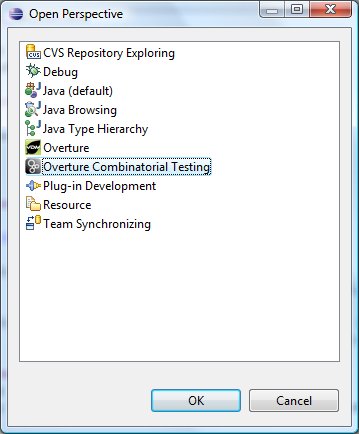
\includegraphics{screenDumps/selectPerspective.png}}
\caption{Select Combinatorial Testing Perspective\label{fig:CTSelectperspective}}
\end{center}
\end{figure}

\begin{figure}[htb]
\begin{center}
\resizebox{\textwidth}{!}{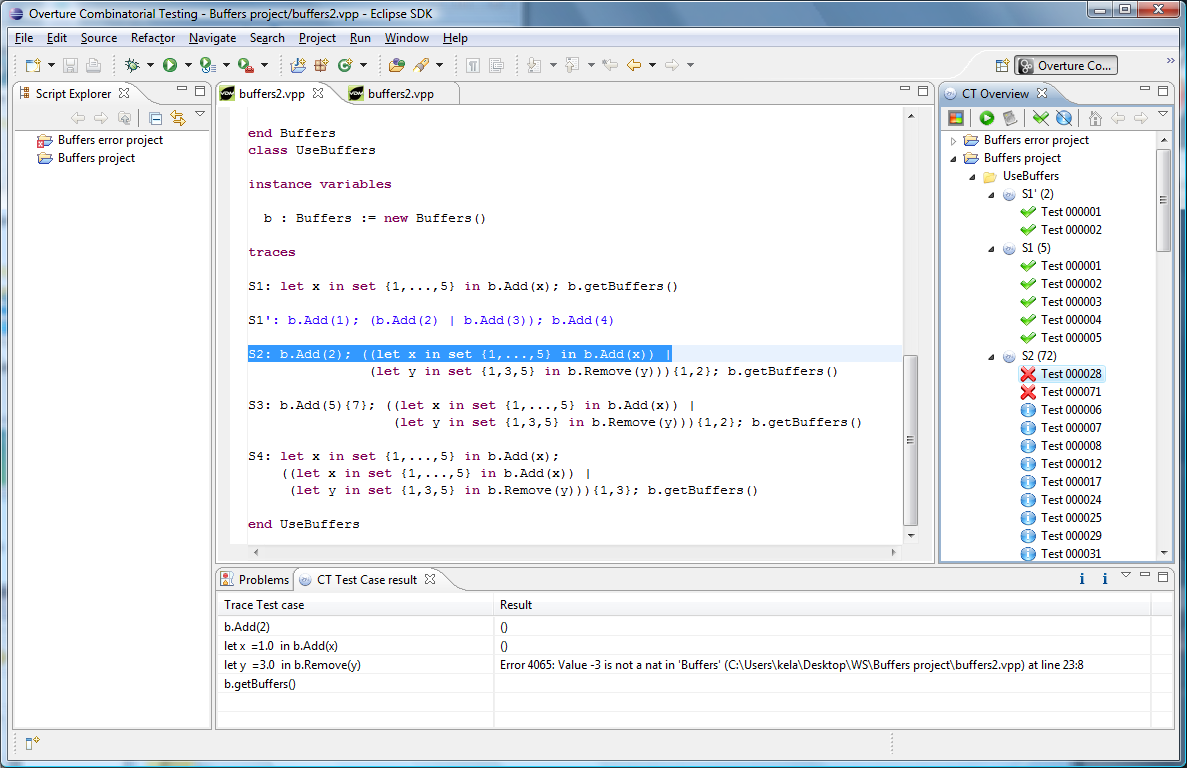
\includegraphics{screenDumps/CTOverview.png}}
\caption{Combinatorial Testing Perspective\label{fig:CTperspective}}
\end{center}
\end{figure}

On the right-hand-side of Figure~\ref{fig:CTperspective} there is a
browser with the title ``CT Overview'' with the projects that contain
all projects and all classes present in each project with a VDM++
model that contains trace definitions.  At the
othermost level it contains projects. At the second level one will find
a list of all the classes that are included in the project that
contains trace definitions. At the third level the trace definitions
inside each class is present. Finally at the fourth level the test
cases that each are expanded from a trace definition is present. The
number of test cases is listed after the name of the trace definition.

When the perspective is opened it will automatically attempt to expand
all the trace definitions in the projects that are open. In
rare cases run-time errors can appear in the expansion process. If
this happens these will be listed in the ``problems'' view in Eclipse
and the source view will have an error icon with the corresponding
line in the trace definition that cannot be expanded. This is exactly
the same as if syntax or type errors are discovered. In
Figure~\ref{fig:ExpandProblems} an example of a problems that can
occur in the process of expanding trace definitions into a collection
of test cases.

\begin{figure}[htb]
\begin{center}
\resizebox{\textwidth}{!}{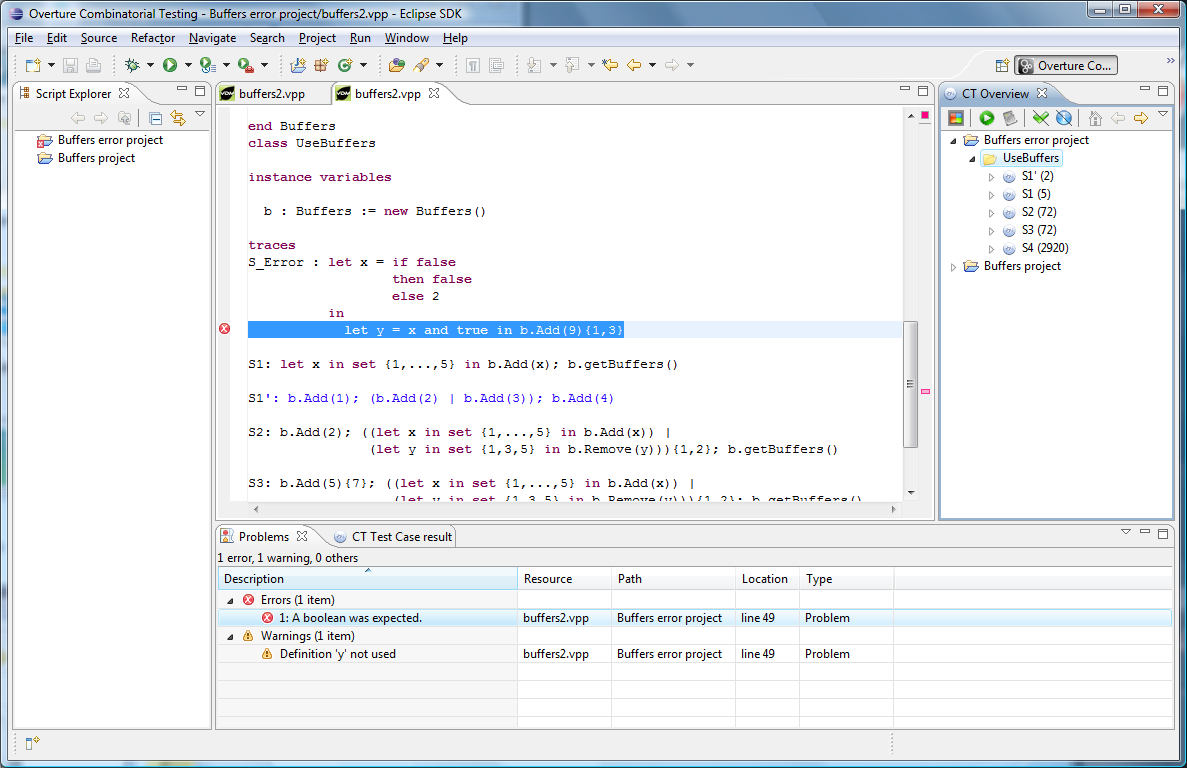
\includegraphics{screenDumps/CTOverviewProblems.png}}
\caption{Example for a problem detected in expanding test cases\label{fig:ExpandProblems}}
\end{center}
\end{figure}

\begin{figure}[htb]
\begin{center}
\resizebox{.3\textwidth}{!}{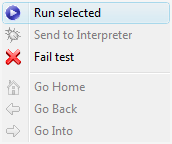
\includegraphics{screenDumps/ContextMenuRun.png}}
\caption{Menu coming up by right-clicking in the CT browser\label{fig:CTmenu}}
\end{center}
\end{figure}

Note in the figure that there is a zero in brackets after the
\texttt{DD} trace definition name in the CT Overview part of
eclipse. This indicates the number of test cases that it has been
expanded to and none gets produced when the expansion results in an
error like in this case. In all cases the number in brackets after the
name of a trace definition indicates the number of test cases that has
been generated.

At all elements in the ``CT Overview'' browser it is possible to right click
and then select the ``Run selected'' option (see the menu in
Figure~\ref{fig:CTmenu}).  As a consequence all the test cases
under the selected item will be executed. 

As an alternative to ``run selected'' one can select the ``Run all''
entry at the top of the ``CT Overview'' browser since that will run
all the test cases in all the active projects. In case any
of the test cases are able to discover errors in the VDM++ model the
trace definitions with these test cases are opened in the browser with a
red cross over them indicating a \emph{fail} verdict for that test
case.  In each of these cases an error have been discovered in the
VDM++ model. It makes sense to fix these errors before proceeding with
using the remaining functionality in the CT perspective. Thus it is
possible to move over to debugger perspective with a selected test
case\footnote{This feature is not yet available though because the
  debugger perspective in Overture is still under development.}. In this
perspective it will be much easier to find out why a particular test
case does not behave as expected.

Different icons are used to illustrate the verdict in a test
case. These are:
\begin{description}
\item[\hspace{-1.8mm}
\raisebox{-0.8mm}{
\includegraphics[width=0.03\textwidth]{icons/unknownWhiteBG.png}}:]
  This icon is used to indicate that the test case has not yet been executed.
\item[\hspace{-1.8mm}
\raisebox{-0.8mm}{
\includegraphics[width=0.03\textwidth]{icons/okBigWhiteBG.png}}:] This icon is used to indicate that the test case has a pass
  verdict.
\item[\hspace{-1.8mm}
\raisebox{-0.8mm}{
\includegraphics[width=0.03\textwidth]{icons/undeterminedBigWhiteBG.png}}:] This icon is used to indicate that the test case has an inconclusive
  verdict.
\item[\hspace{-1.8mm}
\raisebox{-0.8mm}{
\includegraphics[width=0.03\textwidth]{icons/faildBigWhiteBG.png}}:]
This icon is used to indicate that the test case has a fail verdict.
\item[\hspace{-1.8mm}
\raisebox{-0.8mm}{
\includegraphics[height=10pt]{screenDumps/skippedIndication.png}}:] 
If test cases result in a run-time error other test cases with the
same prefix will be filtered away and thereby skipped by in the test
execution. The number of skipped test cases is indicated after number
of test cases for the trace definition name. 

\end{description}

\begin{figure}[htb]
\begin{center}
\resizebox{.5\textwidth}{!}{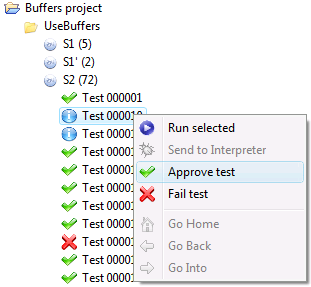
\includegraphics{screenDumps/ContextMenuSkippedApprove.png}}
\caption{Menu for manual selecting verdict in the CT browser\label{fig:CTmanual}}
\end{center}
\end{figure}

Once no more errors can be discovered directly using the CT feature it
is possible to manually step through the test cases individually. When
a test case is selected in the CT Overview browser the contents of the
test case and the corresponding output from the interpreter will be shown in the
``CT Test case result'' window. It is possible to move through the
list of test cases and their results in the ``CT Overview'' browser
and whenever a test case is spotted where the verdict made by the
automatic CT testing analysis is wrong it is possible to change it by
right clicking on the test case and selecting the right verdict
manually (see the menu in Figure~\ref{fig:CTmanual}).  In this process
the tool will skip all test cases that have been filtered away in the
process because these does not supply any new information. In
Figure~\ref{fig:CTmanual} you can also see different icons (\hspace{-1.8mm}
\raisebox{-0.8mm}{
\includegraphics[width=0.03\textwidth]{icons/okFilter16WhiteBG.png}}
and \hspace{-1.8mm}
\raisebox{-0.8mm}{
\includegraphics[width=0.03\textwidth]{icons/undeterminedFilter16WhiteBG.png}}
at the top
that enables filtering away of test cases that have a pass verdict as
well as test cases that have an inconclusive verdict in the lists of
test cases shown in the browser. This can be convenient to use when
one have a large number of test cases and one wish to focus first on a
particular kind of verdicts. Finally it is also possible to sort the
test cases such that all the failed test cases are shown first,
followed by the inconclusive ones and finally the passed ones. This
is done with the sorting icon at the top of the ``CT Overview''
browser (%\hspace{-1.8mm}
\raisebox{-0.8mm}{
\includegraphics[width=0.03\textwidth]{icons/sort16WhiteBG.png}}). 

After running all the test cases selected it is also possible to jump
over to the test coverage information perspective of Overture in order
to be able to see the details of the coverage of the VDM++
model\footnote{This feature is not yet available because the test
  coverage perspective is not yet enabled in Overture.}. Here the user
may be able to detect uncovered parts of the VDM++ model and this can
give inspiration to defining new trace definitions that we will able
to explore more parts of the VDM++ model.

\begin{figure}[htb]
\begin{center}

\resizebox{0.3\textwidth}{!}{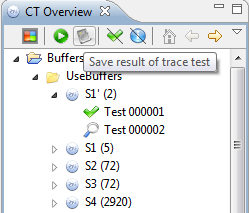
\includegraphics{screenDumps/SaveButton.png}}
%\resizebox{0.1\textwidth}{!}{
\includegraphics{icons/saveWhiteBG.png}}
\caption{Icon for ``Save results of trace test''\label{fig:saveicon}}
\end{center}
\end{figure}

Finally a regression test environment that can be used subsequently
for testing the VDM++ model when further changes are made can be
produced by pressing the small ``save results of trace test'' icon
(see Figure~\ref{fig:saveicon}) at the top of the ``CT Overview
browser''. When this is done argument files (with the \texttt{.arg}
extension) are produced for all test cases and corresponding result
files (with the \texttt{.res} extension) are produced. The root path
of all these test case is determined by the user in a small menu that
comes up when the icon is pressed (see
Figure~\ref{fig:saveresults}). The test cases and their results will
then be produced in a directory structure relative to root for the
project, the class they originally came from and finally the name of
the trace definition.

\begin{figure}[htb]
\begin{center}
\resizebox{0.3\textwidth}{!}{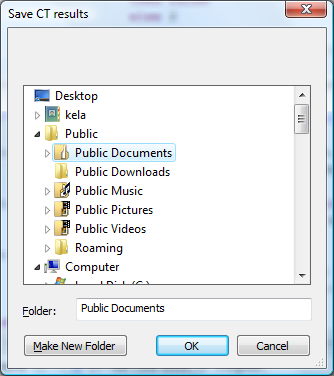
\includegraphics{screenDumps/SaveSelectFolder.png}}
\caption{Determining the root for where to save files\label{fig:saveresults}}
\end{center}
\end{figure}

\subsubsection{Toolbox selection}
The toolbox used when testing the test cases can be selected from two the two supported tools:
\begin{itemize}
    \item Overture VDMJ
	\item The VDM Toolbox v8.2 or later.
\end{itemize}
To select a toolbox the dropdown menu in the CT Overview is used. It
is marked as a down pointing triangle. The menu is shown in
Figure~\ref{fig:toolboxSelectVDMTools}. When selecting a new toolbox
the CT Overview will be reset. If VDM Tools is chosen a dialog asking
for the VDM Tools \texttt{(vppgde.exe})\footnote{Only the Graphical
version of VDM Tools is supported so at the moment please do not
select \texttt{vppde}.} will pop-up asking for the path to the file.

\begin{figure}[htb]
\begin{center}
\resizebox{0.3\textwidth}{!}{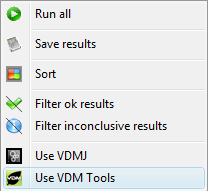
\includegraphics{screenDumps/DropDownMenuUseVDMTools.png}}
\caption{Select Toolbox type.\label{fig:toolboxSelectVDMTools}}
\end{center}
\end{figure}


\section{The command-line interface}\label{sec:command}

In addition to the graphical user interface it is possible to make use
of a command-line version of this tool. This is done from a command
line using the following command:

\begin{alltt}
java -classpath \textit{paths} org.overture.traces.jar \textit{options} \textit{specfiles}
\end{alltt}
\noindent where the options that are enables are:

\begin{description}
\item[-outputPath:] This will be the starting path for all the generated
  test cases and result placed in respectively \texttt{.arg} and
  \texttt{.res} files.
\item[-c:] Followed by a common separated list of the names of the 
  classes that one would like the
  expansion for. If this option is not used all classes will be
  expanded and test cases will be executed.
\item[-max:] Maximum iterations used for star (\texttt{*}) and plus
  (\texttt{+}) in expansion of traces including these operators.
\item[-toolbox:] The VDM++ interpreter which should be used is
     selected here. The options are:
\begin{description}
 \item[VDMTools:] Requires VDMTools to be installed and an additional option
      \texttt{-VDMToolsPath} to be set to the directory with
      the executable file.
 \item[VDMJ:] Requires VDMJ.jar to be in the class path\footnote{In
 the current version of the tool VDMJ is significantly faster than
 using VDMTools.}.
 \end{description}
\end{description}

The command-line version of CT can be fetched as:
\begin{quote}
\url{http://mt.lausdahl.com/CT/org.overture.traces-Cmd_release_v1.zip}
\end{quote}

\noindent This includes a small \texttt{TestRun.bat} file and the buffers
example from the appendix of this user manual as well. 

\subsection{Example of usage}

\begin{alltt}
java -classpath \textit{dirs} org.overture.traces.jar 
     -outputPath c:\back  
     -c A,B 
     -max 3 
     -toolbox VDMJ 
     a.vpp,b.vpp
\end{alltt}

This kind of usage will result in the trace definitions from the
classes \texttt{A} and
\texttt{B} being expanded and tested with the VDMJ interpreter. The
argument and result files will be placed in the \texttt{c:\back A} and
\texttt{c:\back B} directories. There will be one subdirectory here for
each of the named trace definitions and each of these directories will
have one argument file and one result file per test case.

\newpage
\bibliographystyle{newalpha}
\bibliography{dan}
 
\newpage
\appendix
\section{The Buffers Example in Full}\label{app:buffers}

\begin{lstlisting}
class Buffers

instance variables

  b1 : nat := 0;
  b2 : nat := 0;
  b3 : nat := 0;

inv b1 + b2 + b3 <= 40 and b1 <= b2 and b2 <= b3 and b3 - b1 <= 15

operations

public Add: nat ==> ()
Add(x) ==
  if x + b1 < b2
  then b1 := b1 + x
  elseif b2 + x <= b3
  then b2 := b2 + x
  else b3 := b3 + x
pre x <= 5 and b1 + b2 + b3 + x <= 40
post b1 + b2 + b3 = b1~ + b2~ + b3~ + x;

public Remove: nat ==> ()
Remove(x) ==
  if x + b2 <= b3 
  then b3 := b3 - x
  elseif x + b1 <= b2
  then b2 := b2 - x
  else b1 := b1 - x
pre x <= 5 and x <= b1 + b2 + b3
post b1 + b2 + b3 + x = b1~ + b2~ + b3~;

public getBuffers: () ==> nat * nat * nat
getBuffers() ==
  return mk_(b1,b2,b3)

end Buffers
\end{lstlisting}
\newpage

\begin{lstlisting}
class UseBuffers

instance variables

  b : Buffers := new Buffers()

traces

S0: let x = if false then false else 2 in let y = x and true in b.Add(9){1,3}

S1: let x in set {1,...,5} in b.Add(x); b.getBuffers()

S1a: b.Add(1); (b.Add(2) | b.Add(3)); b.Add(4)

S1b: b.Add(1){1,3} 

S2: b.Add(2); ((let x in set {1,...,5} in b.Add(x)) |
               (let y in set {1,3,5} in b.Remove(y))){1,2}; b.getBuffers()

S3: b.Add(5){7}; ((let x in set {1,...,5} in b.Add(x)) |
                  (let y in set {1,3,5} in b.Remove(y))){1,2}; b.getBuffers()

S4: let x in set {1,...,5} in b.Add(x); 
    ((let x in set {1,...,5} in b.Add(x)) |
     (let y in set {1,3,5} in b.Remove(y))){1,3}; b.getBuffers()

end UseBuffers
\end{lstlisting}

\newpage
\section{A Clean Installation}\label{app:install}

This appendix describes how to install the combinatorial testing
feature on top of Eclipse and Eclipse itself and the other tools it
may be dependent upon.

Since this feature has a graphical user interface that is built on top
of the Eclipse development environment let us start by installing a
clean version of that. At
\url{http://www.eclipse.org/downloads/packages/eclipse-classic-341/ganymedesr1}
the classic Eclipse version 3.4.1 can be installed. So if we wish for
example to install on Windows you shall download
\texttt{eclipse-SDK-3.4.1-win32.zip}. If this zip file is unpacked you
will get a new eclipse directory with the files shown in
figure~\ref{fig:eclipsefiles}. 

\begin{figure}[htb]
\begin{center}
\resizebox{0.6\textwidth}{!}{\includegraphics{screenDumpsPGL/eclipsefiles.png}}
\caption{The files availble once eclipse have been unpacked.\label{fig:eclipsefiles}}
\end{center}
\end{figure}

Having installed Eclipse you can now start up
\texttt{eclipse.exe}. The first time this is started up the user will
have to decide where the standard workspace is to be placed and need
to close a welcome window. Then the screen should look like in
figure~\ref{fig:eclipsefirst}. 

\begin{figure}[htb]
\begin{center}
\resizebox{0.9\textwidth}{!}{\includegraphics{screenDumpsPGL/eclipsefirst.png}}
\caption{Startup of Eclipse.\label{fig:eclipsefirst}}
\end{center}
\end{figure}

In order to add the Combinatorial Testing feature you need to select
\texttt{Help -> Software update} as shown in
figure~\ref{fig:eclipseupdate}.

\begin{figure}[htb]
\begin{center}
\resizebox{0.9\textwidth}{!}{\includegraphics{screenDumpsPGL/eclipseupdate.png}}
\caption{Updating Eclipse with additional plug-ins.\label{fig:eclipseupdate}}
\end{center}
\end{figure}

A new window will open up when this is done and here one needs to go
to the ``Available Software'' pane and then click the ``Add Site...''
button. Then you type in the URL for the updatesite as shown in
figure~\ref{fig:CTupdate}. 

\begin{figure}[htb]
\begin{center}
\resizebox{0.9\textwidth}{!}{\includegraphics{screenDumpsPGL/CTupdate.png}}
\caption{Adding the Combinatorial Testing Updatesite.\label{fig:CTupdate}}
\end{center}
\end{figure}

In this installation process you need to accept the license agreements
for a number of other plug-ins that the combinatorial testing plug-in
depends on. Once this have been installed you need to restart Eclipse as it is
suggesting. This completes the actual installation process. Now the
porcess is to start by producing an Overture project. This is done by
selecting \texttt{File -> New -> Other}. The screen should now look at
in figure~\ref{fig:projectopen}.

\begin{figure}[htb]
\begin{center}
\resizebox{0.7\textwidth}{!}{\includegraphics{screenDumps/projectopen.png}}
\caption{Producing an Overture project.\label{fig:projectopen}}
\end{center}
\end{figure}

A new window for wizards will come up. Here you shall selecte the
Overture Project Wizard as illustrated in figure~\ref{fig:overtureprojectwizard}.

\begin{figure}[htb]
\begin{center}
\resizebox{0.4\textwidth}{!}{\includegraphics{screenDumpsPGL/overtureprojectwizard.png}}
\caption{Selecting the Overture Project wizard.\label{fig:overtureprojectwizard}}
\end{center}
\end{figure}

Let us now create a project for the buffers example used in this user
manual. So we will get a screen similar to the one presented in
figure~\ref{fig:buffersproject}. 

\begin{figure}[htb]
\begin{center}
\resizebox{0.6\textwidth}{!}{\includegraphics{screenDumpsPGL/buffersproject.png}}
\caption{Creating the Buffers Project wizard.\label{fig:buffersproject}}
\end{center}
\end{figure}

When ``Finished'' is pressed a new small window will pop up and ask if
you wish to use the Overture perpsective. Here the answer is yes. Now
we can either create a new VDM file in this workspace or we can copy
an existing VDM++ file into the new buffers project we have
created. That can be done by taking the \texttt{buffers2.vpp} file and
copying it. If the mouse is right-clicked in the ``Script Explorer''
area it is then possible to select ``paste''. Now the window should
look like figure~\ref{fig:buffersopened} when the buffers2.vpp file have been selected.

\begin{figure}[htb]
\begin{center}
\resizebox{\textwidth}{!}{\includegraphics{screenDumpsPGL/buffersopened.png}}
\caption{Opening the Buffers Project.\label{fig:buffersopened}}
\end{center}
\end{figure}
 
Now the Overture Combinatorial Testing perspective can be opened as
explained in section~\ref{sec:CTperspective}.

\end{document}
